\documentclass{beamer}
\usepackage{caption}
\usepackage{wrapfig}
\usepackage[parfill]{parskip}
\usepackage{amsfonts}
\usepackage{braket}

% For more themes, color themes and font themes, see:
% http://deic.uab.es/~iblanes/beamer_gallery/index_by_theme.html
%
\mode<presentation>
{
  \usetheme{CambridgeUS}       % or try default, Darmstadt, Warsaw, ...
  \usecolortheme{default} % or try albatross, beaver, crane, ...
  \usefonttheme{serif}    % or try default, structurebold, ...
  \setbeamertemplate{navigation symbols}{}
  \setbeamertemplate{caption}[numbered]
} 

\usepackage[english]{babel}
\usepackage[utf8x]{inputenc}
\usepackage{chemfig}
\usepackage[version=3]{mhchem}
\usepackage{braket}
\definecolor{darkred}{rgb}{0.8,0,0}
\definecolor{Blue}{rgb}{0.2,0.2,0.7}
% On Overleaf, these lines give you sharper preview images.
% You might want to `comment them out before you export, though.
\usepackage{pgfpages}
\pgfpagesuselayout{resize to}[%
  physical paper width=8in, physical paper height=6in]

\def\bone{\mathbf{1}}
\def\b0{\mathbf{0}}
\def\bx{\mathbf{x}}
\def\by{\mathbf{y}}
\def\bz{\mathbf{z}}
\def\ba{\mathbf{a}}
\def\bb{\mathbf{b}}
\def\bc{\mathbf{c}}
\def\bd{\mathbf{d}}
\def\be{\mathbf{e}}
\def\bh{\mathbf{h}}
\def\bm{\mathbf{m}}
\def\bp{\mathbf{p}}
\def\bq{\mathbf{q}}
\def\br{\mathbf{r}}
\def\bs{\mathbf{s}}
\def\bft{\mathbf{t}}
\def\bv{\mathbf{v}}
\def\bg{\mathbf{g}}
\def\bk{\mathbf{k}}
\def\bu{\mathbf{u}}
\newcommand{\cF}{\mathcal{F}}
\newcommand\diff{\mathrm{d}}
\newcommand{\cG}{\mathcal{G}}
\newcommand{\Naniso}{N_{\text{aniso}}}
\newcommand{\Niso}{N_{\text{iso}}}
\def\bf{\boldsymbol}


\setbeamerfont{itemize/enumerate subbody}{size=\scriptsize}
\setbeamerfont{caption}{size=\tiny}


% Here's where the presentation starts, with the info for the title slide
\title{A Brief Introduction to Deep Learning and Computer Vision}
\author{J.S. Blum}
\institute{Department of Radiology, Washington University in St. Louis School of Medicine}
\date{\today}


\setbeamerfont{itemize/enumerate body}{size = \tiny}
\setbeamerfont{itemize/enumerate subbody}{size=\tiny} %to set the body size


\begin{document}

\begin{frame}[plain]
    \titlepage
  \end{frame}

  
% These three lines create an automatically generated table of contents.
\begin{frame}[plain]{Outline}
  \tableofcontents
\end{frame}


\section{About Me}
\begin{frame}[plain]{About Me}


    \begin{enumerate}
        \item \textbf{About:} \mbox{}\\ I am a researcher at the Mallinckrodt Institute of Radiology in Washington University in Saint Louis. I received a BA in Applied Mathematics and Statistics at WashU, advised by Sheng-Kwei Song (Radiology) and Donsub Rim (Mathematics).  \mbox{}\\ \textbf{\textit{Github: @jacobblum}}
        \item \textbf{Research Interests:} \mbox{}\\ My interests are in inverse problems and computational applications in medical imaging: coupled-physics imaging (NMR/dMRI), proton dynamics, deep learning, high performance computing.
        \item \textbf{Some Selected Publications/ Software:} 
        
        \begin{itemize}
            \item \textbf{simDRIFT: a software package for massively parallel forward simulation of diffusion weighted MRI on biophysically accurate tissue systems} \mbox{}\\ \textit{J. Open Source Softw. (2023)}
            \item \textbf{Diffusion basis spectrum imaging provides insights into cervical spondylotic myelopathy pathology} \mbox{}\\ \textit{Neurosurgery (2022)}
            \item \textbf{Analysis of combined clinical and diffusion basis spectrum imaging metrics predicts the outcome of chronic cervical spondylotic myelopathy following cervical decompression surgery} \mbox{}\\ \textit{J. of Neurosurgery: Spine (2022)}
            \item \textbf{Diffusion Basis Spectrum Imaging Distinguishes High Grade Glioma Treatment Effect From Tumor Progression} \mbox{}\\ \textit{Neuro-Oncology (2023)}
            \item \textbf{Utility of Diffusion Basis Spectrum Imaging in Quantifying Baseline Disease Severity and Prognosis of Cervical Spondylotic Myelopathy} \mbox{}\\ \textit{Spine (2022)}
        
        
        \end{itemize}
    \end{enumerate}
    
\end{frame}


\section{Image Processing}
\begin{frame}[plain]{What Are Images: ND-Arrays}
\begin{definition}
    Diverse mathemtaical descriptions of obejcts and images can be unifed by the imaging equation.
    \begin{align}
        \mathbf{g} = \boldsymbol{\mathcal{H}}\mathbf{f}
    \end{align}
    Where $\mathbf{g}$ is the image, $\mathbf{f}$ the imaging object, and $\mathcal{H}$ the imaging system.

    For example ...

    \begin{figure}
        \centering
            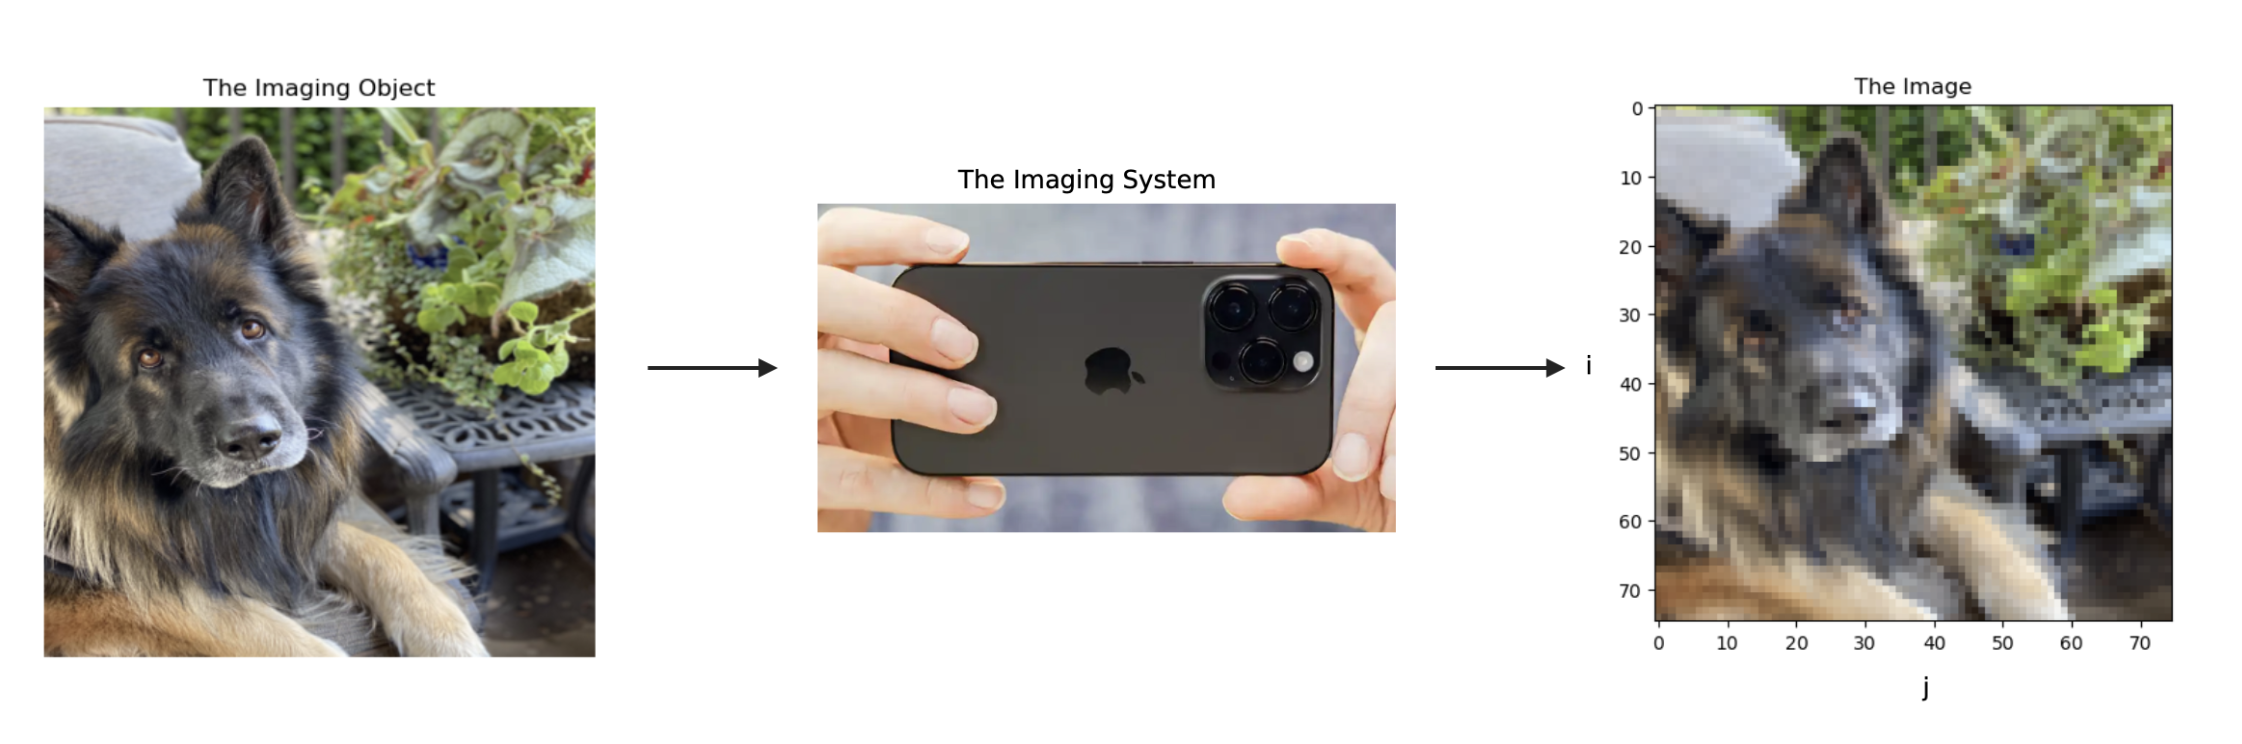
\includegraphics[width = \textwidth]{/Users/jacobblum/Desktop/Computer_Vision/figs/an_imaging_system.png}
            \caption{The Imaging system (a camera) produces a discretized represtnation of the imaging object. Typically, this is can be thought of as a 2D array}
        \end{figure}
    \end{definition}
\end{frame}

\begin{frame}[plain]{What do we do with Images: Image Processing}
    There is an enormous demand for image processing in a diverse range of application areas including biomedical imaging, autonomous systems, and reomote sensing.
    \begin{figure}
        \centering
            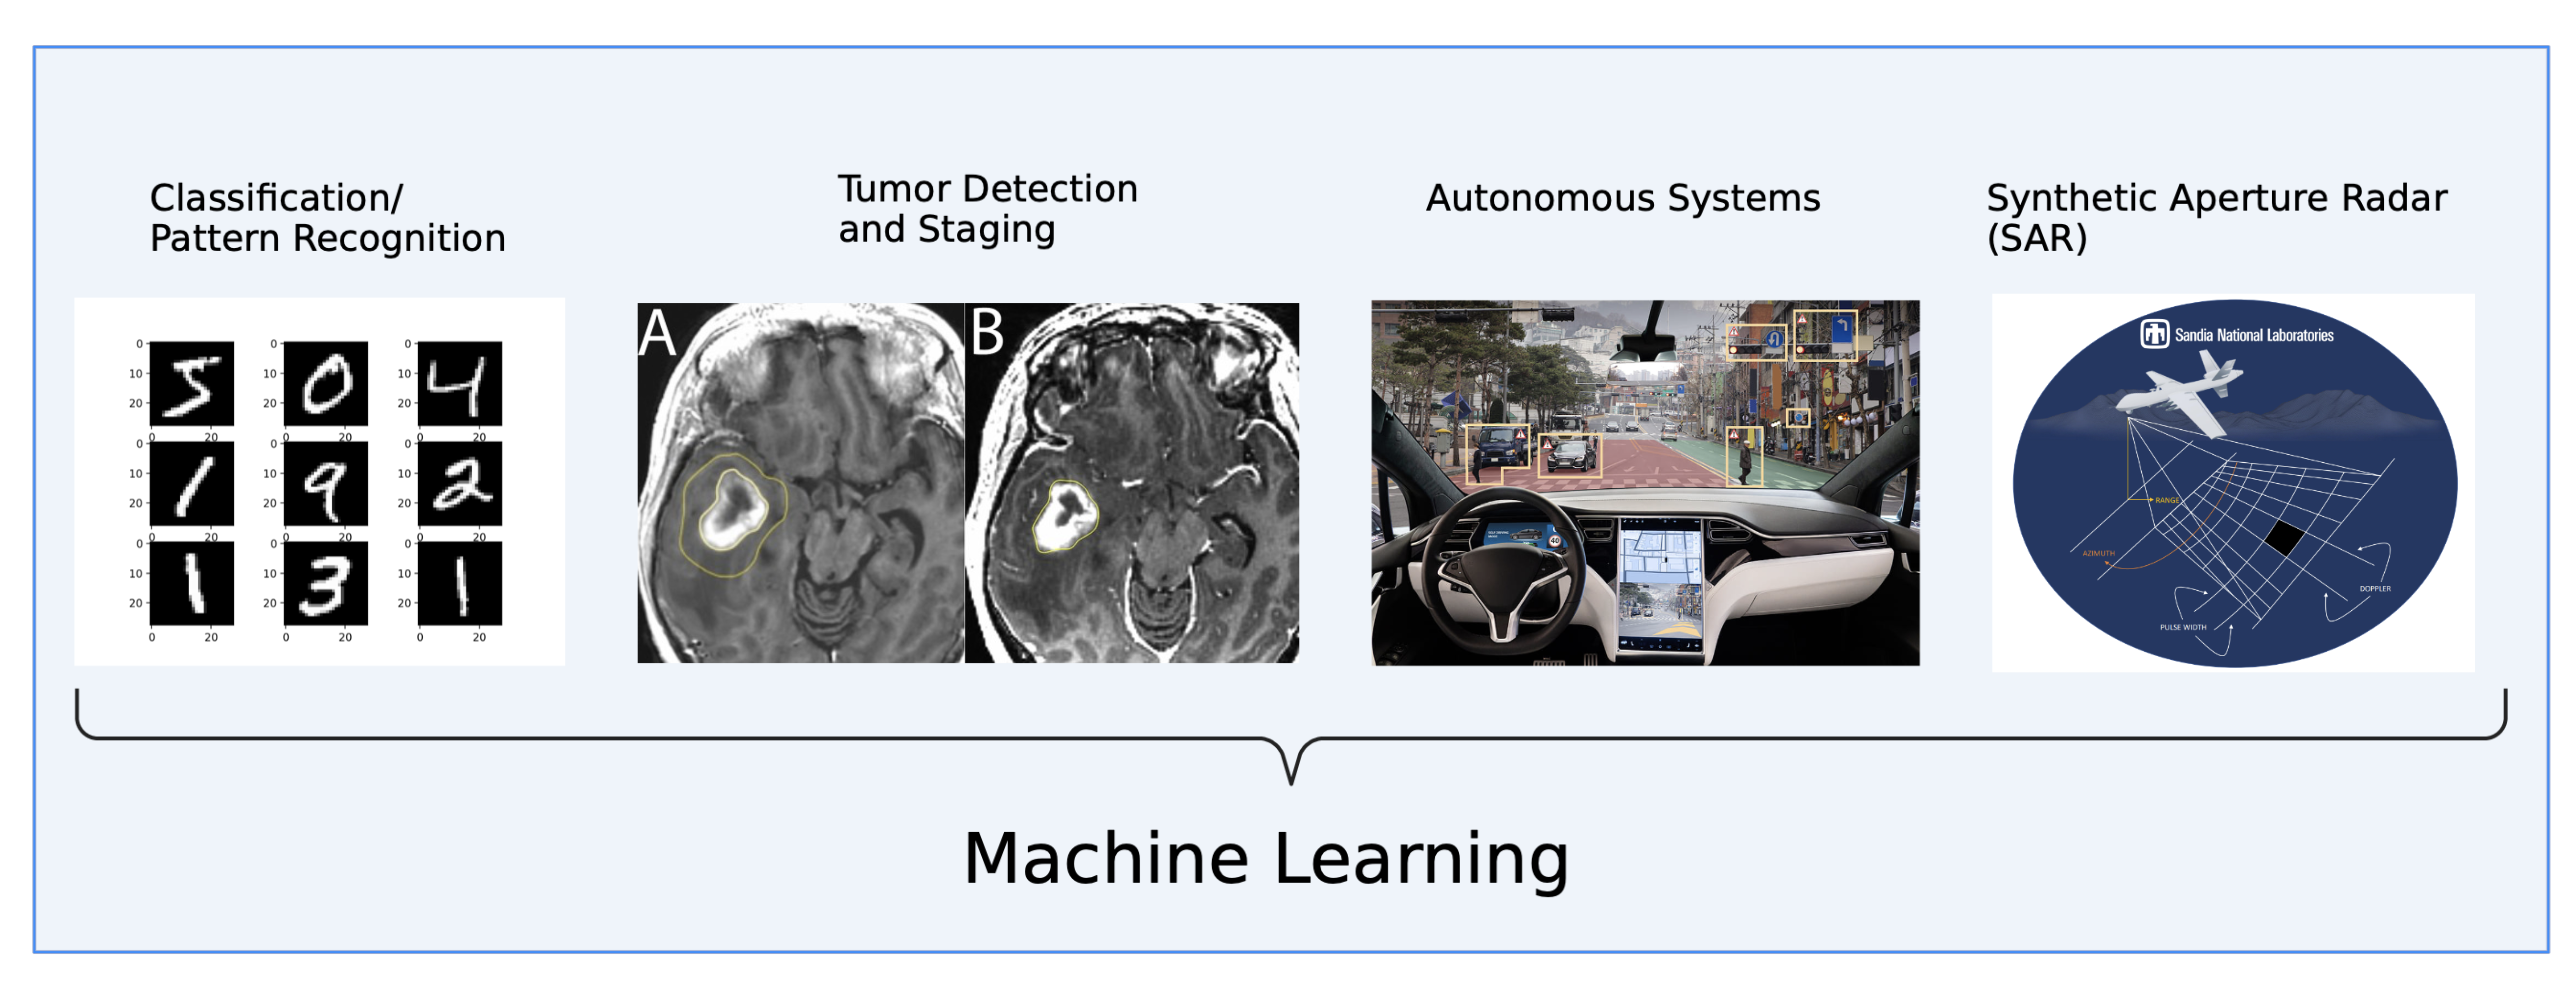
\includegraphics[width = \textwidth]{/Users/jacobblum/Desktop/Computer_Vision/figs/Image Processing.png}
            \caption{(Left) MNIST Dataset, a common benchmark for image classication models; T2W/FLAIR images of GBM with ML guided segmentation; A self driving car using computer vision; A SAR system on a UAV}
        \end{figure}
\end{frame}


\begin{frame}[plain]{Tools for Image Processing}



\end{frame}
\end{document}

